\section{Vision}

\subsection{Code Reuse}

We started off by taking group 3's from last year code.  We chose this group's code because it was written in Java which we were all familiar with allowing us to get to work straight away. Also it was the most understandable, in terms of source code, in comparison to the other vision systems developed in Java.  Their control G.U.I. was also very impressive, being clean and easy to use.  Their vision system had all the necessary elements including grabbing the vision feed, which other teams this year had more trouble with than us.  However, it was running at around 24fps and it was using two colour spaces HSV and RGB to preform thresholding, without any explanation of which values are used for what. 

We also used the barrel distortion correction code from group 5.  Most groups who had barrel distortion correction were using a variant of openCV and so had functions that we couldn't use.  Group 3 had attempted to correct the barrel distortion but had been unsuccessful which is why we used group 5.  It was very effective working straight out of the box.

\subsection{In the Beginning}

After deciding on which code we were going to use we started to realise how unwieldy it was.  Most of the work was being done in an undocumented 700ish line method.  So first thing for us to do was to work out what was going and try and do our best to refactor it to make it more understandable.  We then saw that they were using both hsv and rgb values for thresholding, so we stripped out the hsv checking.  In group 3's code the thresholding was done by moving sliders around to find the optimal values, we changed this so that the thresholding would be based on a click, saving time and effort (this was later removed when Rado's better thesholding technique was introduced).  We then started the work of improving the accuracy and efficiency of their code (DO WE HAVE ANY STATS ON WHAT IS WAS WHEN WE STARTED?).  This included heavy refactoring, new algorithms for all aspects of the system.  All we are using currently is their code for grabbing frames, and some aspects of their G.U.I.

POSSIBLY NEEDS MORE WHY?  SHOULD WE GO INTO MORE DETAIL ON WHAT WE HAVE NOW

\subsection{Integration}

The main advantage of using a previous year�s code was that it allowed us to start planning and coding almost immediately. One of the key parts focused on initially was the creation of �WorldState�. This was a class which held all the current data about the pitch, updated as often as the frame refreshed usually. It was planned to be as easy to use as possible with clear getters and setters for each variable. With this in place strategy would know exactly what data they had available and how to access it giving them an easier time in planning. However, it was not completely clear when we initially started what data we would need and over time the class grew larger and larger, requiring a major refactor which split the WorldState into its different components (two robots, a ball and the pitch). The layout was clear and easy to use and facilitated faster planning and coding, helping us develop as good a robot as possible.

This, however, was our only thought towards integration. It was reasoned that since each sub-system was part of the same application, when another system required more processing time, vision could slow down and give up its processor time to another sub-system. This turned out to be more difficult to implement than we originally anticipated. The problem could have been effectively resolved by researching more in the initial stages of the vision system.

\subsection{Thresholding using RGB}

We implemented a simple, yet very efficient, in terms of accuracy and speed, algorithm to preforms thresholding for specific colours, using only the RGB colours space. This was used for recognition of the objects on the pitch. The method works by noting that red, for example, can be identified as something that has high value of the red channel and low values at the green and blue.  Thus, inspecting a pixel in all three colour channels and using a broather notion of what can really be considered as red, the pixels of the ball are extracted. This notion is best illustrated by the following figure: 

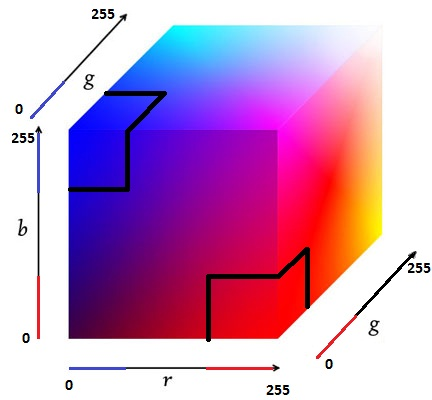
\includegraphics[scale=1]{RGB_Space.jpg} 

Similar technique was used for the other colours, representing the other objects. An example for blue is also illustrated in the figure. We chose RGB for several reasons. It is more intuitive and it produced a faster and more accurate results. Since Java supplies the grabbed frame in RGB, no time is waisted in conversion to other colour spaces. The system could identify the position of the two robots, the ball, and their orientations within 37 fps. For the deciding of how accurate the method was, human oracle testing was used. This involved team members to visually check the validity of the outputs produced by the method, given an observed visual setting. Also, a comprehensive guide was written as a documentation, explaining the workings of the method, so future developers can understand and improve. 

\subsection{Random Sampling for Centroid Calculation}

Centroiding can be strongly affected by noise, even just a few noisy pixels, this was a problem for us because the yellow in the vision feed was quite grey and testing for yellow pixels would capture parts of the robot that weren't yellow.  Applying a noise filtering algorithm was too slow, halving the frame rate, and clustering was a bit too slow for our tastes.  So James came up with a technique to give us the benefits of clustering in linear speed.  Below is an example of how the algorithm works using the yellow T as an example.
\begin{enumerate}
\item Go through frame pixel by pixel, if pixel is identified as yellow then place it one of five bins randomly.
\item Calculate centroid of all five bins.
\item If the centroid of a bin does not lie on a yellow pixel then discard it, thus removing the noisy pixels.
\item Take the mean of the remaining centroids and set this to be the centroid of the object, in this case the yellow T.
\item If all bins were discarded then keep the centroid where it was.
\end{enumerate}

The case of all the bins being discarded is a rare one, as there are very few noisy pixels compared to non noisy pixels.  This method was very fast, we only lost a couple of fps from the processing.  Using the vision testing system (when it was not well calibrated) it achieved accuracy of around 85\% but through oracle testing it was clear it was far more accurate, nearing 100\%.

\subsection{Vision Testion System}

One of the most important things in any application is the knowledge that the application works as expected. The key to this is having a good testing system. With a testing system you can change your algorithms, using the tests to ensure that they continue to function as desired. Testing the vision system was extremely tricky and required some serious problem solving. The functions were giving us results, but we had no data to test against. The solution was rather elegant: Each time the system is run in the debugging mode, present a freeze frame to the user and ask them to provide the data. This was accomplished by the user clicking the positions of the robots and the ball. For the orientation we had them also click the tip of the T, getting a result accurate to within 5 degrees - an acceptable margin of error. The data was stored as an XML file along with the freeze frame. When it came to running unit tests, either manually or by our build system Jenkins, we simply had to run the single frame through the vision testing system and compare the generated results to the user generated results. If they matched within a certain degree then the test passed. A simple and elegant solution for a complex problem. 

\subsection{Are we happy?}

The vision system overall was excellent. It provided us with extremely accurate and consistent results, as shown by our testing system, and was still fast enough to process every single frame without performance loss. That being said, the vision system was only so good because of the time and effort invested in it. Given the chance to do it again we would change the development in one key way: use Python instead of Java. Python was a much more suitable language for this project and was only avoided due to inexperience with the language. It has access to the SimpleCV library (Java also has access but it is much more difficult to interact with) which would have speeded development by a rather large factor with very similar results. Accuracy could have been increased even further, the only downside being the slightly slower speed. This we feel would have been an acceptable trade off as it would have allowed us to re-assign our manpower much more effectively - a vital task in a smaller team such as our own.





